\documentclass[sigconf]{acmart}
\settopmatter{printacmref=false} % Removes citation information below abstract
%\renewcommand\footnotetextcopyrightpermission[1]{} % removes footnote with conference information in first column
\pagestyle{plain} % removes running headers
\pagestyle{empty}

\usepackage{array}
\usepackage{graphicx}
\usepackage{clrscode}
\usepackage{balance}
\usepackage{subfigure}
\usepackage{multirow}
\usepackage{float}
\usepackage{color}
\usepackage{soul}
\usepackage{mdframed}
\usepackage{amsopn}
\usepackage{mathrsfs}
\usepackage{mathtools}
\usepackage{amsmath}
\usepackage{arydshln}
\usepackage{hyperref}
\usepackage{multicol}
\usepackage{blkarray}
\usepackage{enumerate}
\usepackage{courier}
\usepackage{rotating}
\usepackage{booktabs}
\usepackage{diagbox}
\usepackage{fancybox}
\usepackage{minibox}
\usepackage{cases}
\usepackage{listings}
\lstset{
  basicstyle=\ttfamily,
  breaklines=true,
  postbreak=\mbox{\textcolor{red}{$\hookrightarrow$}\space},
}
\usepackage[lined,boxruled,commentsnumbered,linesnumbered]{algorithm2e}
\usepackage{bm}


\newcommand{\ylcomment}[1]{\textcolor{blue}{[#1---yl]}}

\DeclareRobustCommand{\hlblue}[1]{{\sethlcolor{blue}\hl{#1}}}
\DeclareRobustCommand{\hlgreen}[1]{{\sethlcolor{green}\hl{#1}}}
\DeclareRobustCommand{\hlred}[1]{{\sethlcolor{red}\hl{#1}}}

\newcommand{\argmin}{\operatornamewithlimits{argmin}}
\newcommand{\argmax}{\operatornamewithlimits{argmax}}
\newcommand{\minimize}{\operatornamewithlimits{minimize}}
\newcommand{\maximize}{\operatornamewithlimits{maximize}}
\newcommand{\random}{\operatornamewithlimits{random}}
\newcommand{\suchthat}{\operatornamewithlimits{s.t.}}
\newcommand{\rank}{\operatornamewithlimits{rank}}
\newcommand{\trace}{\operatorname{tr}}
\newcommand{\vectorize}{\operatornamewithlimits{vec}}
\newcommand{\diag}{\operatornamewithlimits{diag}}
\newcommand{\bdf}{\operatornamewithlimits{bdf}}
\newcommand{\bbdf}{\operatornamewithlimits{bbdf}}
\newcommand{\rbbdf}{\operatornamewithlimits{rbbdf}}
\newcommand{\hdline}{\hdashline[2pt/2pt]}
\newcommand{\vdline}{\vdashline[2pt/2pt]}
\newcommand{\vdl}{;{2pt/2pt}}
\newcommand{\tabincell}[2]{\begin{tabular}{@{}#1@{}}#2\end{tabular}}

%\setcopyright{rightsretained}
%\acmDOI{10.475/123_4}
%\acmISBN{123-4567-24-567/08/06}
%\acmConference[SIGIR'19]{}{}{July 21-25, 2019, Paris, France}
%\acmYear{2018}
%\copyrightyear{2018}
%\acmPrice{15.00}
\usepackage{algorithm}
\usepackage{algorithmic}
\begin{document}

\title{Movie Recommendation System on MovieLens Dataset}

\author{Han Wu \ \ Ningyuan Zhang \ \ Lemin Wu \ \ Zhe Huang}
\affiliation{
 \institution{Department of Computer Science, Rutgers University}
}
\email{  {han.hw.wu,  ningyuan.zhang,  lemin.wu,  quincy.huang} @rutgers.edu}

%%%%%%%%%%%%%%%%%%%%%%%%%%%%%%%%%%%%%%%%%%%%%%%%

\maketitle

%%%%%%%%%%%%%%%%%%%%%%%%%%%%%%%%%%%%%%%%%%%%%%%%%%%
\section{Introduction}
Recommender system has been widely used in many fields. It can be seen as a platform or engine which predicts user preferences and can recommend items to a user based on them. Recommender system can be used as playlist generators for movies or videos in YouTube or Netflix. It can achieve product recommender in Amazon or eBay. And it can also provide news recommendation in Bloomberg.

The problem this project tries to solve is a movie rating prediction problem. The dataset we have has some ratings of some users to some movies, However, there are also many vacancies. Our goal is to predict these vacancies and recommend items to users based on these predictions. 

Many models can be used in recommender system. We decide to use collaborative filtering and latent factor model in this project. In collaborative filtering, we use user-user collaborative filtering and item-item collaborative filtering. In latent factor models, we use basic latent factor model, latent factor model with bias, and latent factor model with temporal biases. Different models have different pros and cons. We compare them with each other.

The experimental results will be described below in details.


\section{Related Work}\label{sec:related}
Here are the three types of recommendation systems that are frequently used. 
\item{1.Content-Based Filtering}
\item{The Content-Based Recommender relies on the similarity of the items being recommended. The basic idea is that if you like an item, then you will also like a “similar” item.The concepts of Term Frequency (TF) and Inverse Document Frequency (IDF) are used to pick important features such as author/actor/director to create an item profile for each movie. Then, the user profile vectors are also created based on his actions on previous attributes of items and the similarity between an item and a user is also determined in a similar way.}
\item{2.Collaborative Filtering}
\item{The Collaborative Filtering Recommender is entirely based on the past behavior and not on the context. More specifically, it is based on the similarity in preferences, tastes and choices of two users. It analyzes how the tastes of one user are similar to another and makes recommendations based on that. In User-User Collaborative Filtering, we find look-alike users based on similarity and recommend movies which the first user has chosen in the past. Item-Item Collaborative Filtering is quite similar to previous algorithm, but instead of finding similar users, we try to find similar movies.}
\item{3.Matrix Factorization}
\item{In the previous attempt, rating matrices may be overfitted to noisy representations of user tastes and preferences. In addition to this, it doesn’t scale well to extremely large datasets because it needs a lot of computations to make recommendations. So, we can apply Dimensionality Reduction techniques to derive the tastes and preferences from the raw data, which is also known as low-rank matrix factorization.}


\section{Preliminaries}\label{sec:preliminary}
The dataset we use is from MovieLens Latest Datasets. MovieLens is an online movie-rating website. People can rate movies they watched before in this website. There are many rating datasets on this website. Based on our hardware infrastructure and computing resources, we choose the ml-latest-small dataset. The last update is Sept. 2018. It has over 100000 ratings, which is applied to 9724 movies by 610 users. There are four files in this dataset --- links.csv, movies.csv, ratings.csv, tags.csv. We mainly focus on ratings.csv.

The dataset needs to be separated into two parts --- training set and test set. The training set contains 80\% of the data. The test set contains 20\% of the data. Two ways are used in our project to split the data. We use train\_test\_split() from sklearn.model\_selection package to directly split the data into 2 parts. We also choose some of users and some of their ratings to get train/test dataset. Training set is used to train the model and test set is used to assess whether the model is good or not.


\section{Problem Formalization}\label{sec:formal}
We can formalize the problem by the following way.\\
X = set of users\\
I = set of movies\\
Utility function $u: X * I \rightarrow R$\\
R = set of ratings in the range [0.5, 5]\\
A sample Utility Matrix can be represented as:\\
$\begin{matrix} 
  & user1 & user2 & user3 \\
movie1 & 0.5 &   & 4\\
movie2 &     & 3 & 5\\
movie3 & 1   &   &  \\
\end{matrix}$\\
\\

The key steps to solve the problem are:\\
1. Create training and validation dataset by splitting the original dataset (the rating in the validation dataset are treated as unknown).\\
2. Predict unknown ratings from the known ones - develop user-based CF model, item-based CF model, basic latent factor model and latent factor model with Biases to conduct rating prediction.\\
3. Evaluate predictions by calculating the MAE and RMSE\\
MAE - Mean Absolute Error\\
\begin{equation*} 
MAE = \frac{1}{n}\sum_{i=1}^n|pred_i - actual_i|\\
\end{equation*} 
RMSE - Root Mean Square Error\\
\begin{equation*} 
RMSE = \sqrt{\frac{1}{n}\sum_{i=1}^n(pred_i - actual_i)^2}\\
\end{equation*} 
4. Create a recommendation list based on predictions for each user\\
5. Evaluate the quality of the recommendation list by calculating precision, recall, F-measure and NDCG. The formulas of these criteria are shown below.\\
$Precision = \frac{tp}{tp+fp}=\frac{|good\_movies - recommended|}{|all-recommended|}\\
Recall = \frac{tp}{tp+fn}=\frac{|good\_movies - recommended|}{|all-good-movies|}\\
F = 2\frac{precision*recall}{precision + recall}\\
NDCG = \frac{DCG}{IDCG}$\\


\section{The Proposed Model}\label{sec:framework}
\subsection{User-User Collaborative Filtering}
\item{The main idea is to find set N of other users whose ratings are similar to x's ratings and create the recommendation list based on them.\\
Firstly, we weight the similarity between each two users. Here we use Cosine similarity measure since Jaccard similarity measure ignores the value of the rating.
\begin{equation} 
sim(x,y)=cos(r_x,r_y)=\frac{r_x.r_y}{||r_x||.||r_y||}
\end{equation}
Next, we move forward to implement prediction for movie i of user x. Let N be the set of K users most similar to x who have rated movie i.
\begin{equation} 
r_{xi}=\frac{\sum_{y\in N}sim(x,y).r_{yi}}{\sum_{y\in N}sim(x,y)}
\end{equation}
At this time, we could recommend movies for each user. 
\begin{algorithm}
\caption{User-User Collaborative Filtering Recommendation}
\label{alg:A}
\begin{algorithmic}
\STATE $rec=\{\}$;\
\FOR{each $u \in users$}
\STATE $Poss\_movie=set()$;\
\STATE $rank=\{\}$;\
\STATE $N=$ the set of top K similar users of $u$;\
\FOR{each $v \in N$}
\STATE $v\_watched=$ movies that $u$ has watched;\
\FOR{each $movie \in v\_watched$}
\IF{$u$ has not watched $movie$} 
\STATE $Poss\_movie$.add($movie$);\
\ENDIF 
\ENDFOR

\ENDFOR
\FOR{each $movie \in Poss\_movie$}

\STATE $score=predict (u,movie)$;\
\STATE $rank.setdefault(movie, 0)$;\
\STATE $rank[movie]=score$;\
\ENDFOR
\STATE  $rec[u]=sorted(rank.items())[0:10]$;\
\ENDFOR
\end{algorithmic}
\end{algorithm}

}

\subsection{Item-Item Collaborative Filtering}
The main idea is to find similar movies of the unknown movie and use these similar movies to predict the unknown one. Then find 10 movies with highest prediction rating to recommend.\\
\\
Firstly, we centered rating by $r_i = r_i - \Bar{r}$.\\
Similar to user-user collaborative filtering, we weight the similarity between each two movies. Here we use Cosine similarity measure since Jaccard similarity measure ignores the value of the rating\\
\begin{equation} 
sim(i,j)=cos(r_i,r_j)=\frac{r_i.r_j}{||r_i||.||r_j||}
\end{equation} 
Next, we move forward to implement prediction for movie i of user x.\\
\begin{equation} 
r_{xi}=\frac{\sum_{j\in N(i;x)}S_{ij}.r_{xi}}{\sum_{j\in N(i;x)}S_{ij}}
\end{equation} 
$S_{ij}$ - similarity of movies i and j\\
$r_{xj}$ - rating of user x on movie j\\
N(i;x) - set of movies rated by x similar to i\\
\\
According to the predictions, we could recommend movies with highest prediction rating for each user.\\

\subsection{Basic Latent Factor Model}
\item{ Latent factor model considers users and movies are related to some latent factors. So, the rating matrix can be factorized as the user matrix and movie matrix. The user matrix relate each user to each factor. The movie matrix relate each movie to each factor. We use $u$ to denote the number of users and $m$ to denote the number of movies. $f$ is used to represent the number of factors. We use $R$, $P$, and $Q$ to denote the rating matrix, user matrix, and movie matrix respectively. So, we have $R=PQ$. The dimension of rating matrix is $u \times m$, while the dimensions of user matrix and movie matrix are $u \times f$, and $f \times m$. We use \boldsymbol{${p_x}$} to represent the latent vector of user $x$. \boldsymbol{${p_x}$} is a row vector of dimension $1 \times f$. We use \boldsymbol{${q_i}$} to denote the latent vector of movie $i$. \boldsymbol{${q_i}$} is a column vector with dimension $f \times 1$. The cost function of this basic latent factor model is
\begin{equation}
    J = \frac{1}{N} \sum_{(x,i) \in R} (r_{xi} - p_x \cdot q_i)^2  + \frac{\lambda_1}{N} \sum_x \| p_x \|^2 + \frac{\lambda_2}{N} \sum_i \| q_i \|^2
\end{equation}
We do summation only on the positions where ratings already exist. $\cdot$ means dot product between vector \boldsymbol{${p_x}$} and vector \boldsymbol{${q_i}$}. $N$ represents the number of all training examples. $\lambda_1$ and $\lambda_2$ are regularization terms to avoid overfitting.

Our goal is to minimize the cost function with respective to $P$ and $Q$ so that we can get the final model.
\begin{equation}
    \min_{P,Q} J
\end{equation}
We use Gradient Descent(GD) to solve the minimization problem. The gradients of parameters are
\begin{equation}
    \frac{\partial J}{\partial p_{xk}} = \sum_{(x,i) \in R} \frac{-2}{N} (r_{xi} - p_x \cdot q_i) q_{ki} + \frac{2\lambda_1}{N} p_{xk}
\end{equation}
\begin{equation}
    \frac{\partial J}{\partial q_{ki}} = \sum_{(x,i) \in R} \frac{-2}{N} (r_{xi} - p_x \cdot q_i) p_{xk} + \frac{2\lambda_2}{N} q_{ki}
\end{equation}
where $k$ denotes the index of factors.

We can also use a vectorized way to calculate the gradients because matrix operations are often faster.
\begin{equation}
    \frac{\partial J}{\partial P} = \frac{-2}{N} ((R - P \cdot Q)*E)\cdot Q^T + \frac{2\lambda_1}{N} P
\end{equation}
\begin{equation}
    \frac{\partial J}{\partial Q} = \frac{-2}{N} P^T \cdot ((R - P \cdot Q)*E) + \frac{2\lambda_2}{N} Q
\end{equation}
In the equations above, $\cdot$ represents dot product between two matrices. $*$ represents element-wise product, where one element in the first matrix multiplies with another element at the same position in the second matrix. $P^T$ means the transpose of matrix $P$. $E$ denotes the existing matrix. $E_{xi} = 1$ if there exists a rating in position $(x,i)$ of matrix $R$.

Once we have the gradients, we need to optimize the parameters. The update rules are
\begin{equation}
    P := P - \alpha \frac{\partial J}{\partial P}
\end{equation}
\begin{equation}
    Q := Q - \alpha \frac{\partial J}{\partial Q}
\end{equation}
where $\alpha$ is the learning rate of this model.

In one iteration, we compute the gradients and update the parameters. We iterate multiple times and finally we get the optimized parameters.

So, this is the basic latent factor model and its working mechanics. The following more complex models are based on it.

}

\subsection{Latent Factor Model with Biases}

In order to boost the basic version of latent factor model, a very effective way is to take the biases of users and movies into consideration. Bias means users' inclination and preference in terms of criteria of movies. For example, a critical viewer is very likely to rate movies lower than average. The bias against movies means some movies are so loved that they normally receive higher ratings than average. By taking bias into account, we can simulate a better model to capture the essence and perfect the choices of recommendation.

As mentioned in the last paragraph, we introduce 3 kinds of bias into the basic model, the overall mean rating $\mu$, the bias $b_x$ for user $x$ and the bias $b_i$ for movie $i$.
\begin{equation}
	r_{xi} = b_{xi} + q_i p_x
\end{equation}
\begin{equation}
	b_{xi} = \mu + b_x + b_i
\end{equation}

The basic idea is using Stochastic Gradient Descent(SGD) to find the parameters that optimize our model.
\begin{equation}
	\begin{split}
	\min_{Q,P} & \sum_{(x,i) \in R} (r_{xi} - (\mu + b_x + b_i + q_i p_x)^2) \\
	& + (\lambda_1 \sum_i \| q_i \|^2 + \lambda_2 \sum_x \| p_x \|^2 + \lambda_3 \| b_x \|^2 + \lambda_4 \| b_i \|^2)
	\end{split}
\end{equation}
The update rules are similar to those above.


\subsection{Latent Factor Model with Temporal Biases}
\item{

The bias of a movie is changing over time. If a movie appears on the movie rating website longer, its rating will become higher. Different movies have different patterns of rating changing. The user bias can also change over time. In this project, we focus on the change of movie bias.

In the dataset, each piece of data has an attribute called timestamp which represents the time of this rating. We use $t'$ to denote the real time. We do not need finest resolution to analyze the temporal effect. So, a reasonable solution is to split the real time $t'$ into some time-based bins\cite{cf-temporal}. We split the timeline into several bins. For a certain range of time, it maps into one bin. The mapping relation can be denoted as $t = Bin(t')$, where $t$ represents the corresponding bin of real time $t'$. $t \in \left\{ 1, 2, \dots, T \right\}$, where $T$ is the number of bins. 

We use $Bu$ to denote the user bias vector whose dimension is $u \times 1$. The element of $Bu$ is $b_x$, which is the bias of user $x$. $Bm$ is used to denote the movie bias matrix. Its dimension is $T \times m$. The element of $Bm$ is $b_{ti}$, which is the bias of movie $i$ in bin-time $t$. We use stochastic gradient descent to deal with the optimization problem. We deal with the rating $r_{xti}$ one by one. $r_{xti}$ represents the rating of user $x$ at bin-time $t$ to movie $i$. For a certain data point $r_{xti}$, the corresponding cost is
\begin{equation}
\begin{split}
    J_{xti} = (r_{xti} - (\mu + b_x + b_{ti} + p_x \cdot q_i))^2 + \lambda_1 \sum_x \| p_x \|^2 \\ + \lambda_2 \sum_i \| q_i \|^2 + \lambda_3 \| Bu \|^2 + \lambda_4 \| Bm \|^2
\end{split}
\end{equation}
We use $\epsilon_{xti}$ to denote $2(r_{xti} - (\mu + b_x + b_{ti} + p_x \cdot q_i))$. For $r_{xti}$, we first calculate the gradients with respect to \boldsymbol{${p_x}$} and \boldsymbol{${q_i}$}.
\begin{equation}
    \frac{\partial J_{xti}}{\partial p_{xk}} = - \epsilon_{xti} q_{ki} + 2 \lambda_1 p_{xk}
\end{equation}
\begin{equation}
    \frac{\partial J_{xti}}{\partial q_{ki}} = - \epsilon_{xti} p_{xk} + 2 \lambda_2 q_{ki}
\end{equation}
These two equations can be vectorized.
\begin{equation}
    \frac{\partial J_{xti}}{\partial p_x} = - \epsilon_{xti} q_i^T + 2 \lambda_1 p_x
\end{equation}
\begin{equation}
    \frac{\partial J_{xti}}{\partial q_i} = - \epsilon_{xti} p_x^T + 2 \lambda_2 q_i
\end{equation}
We then calculate the gradients with respect to $b_x$ and $b_{ti}$ for $r_{xti}$.
\begin{equation}
    \frac{\partial J_{xti}}{\partial b_x} = - \epsilon_{xti} + 2 \lambda_3 b_x
\end{equation}
\begin{equation}
    \frac{\partial J_{xti}}{\partial b_{ti}} = - \epsilon_{xti} + 2 \lambda_4 b_{ti}
\end{equation}
We then update the parameters based on these gradients. The update formulas are
\begin{equation}
    p_x := p_x - \alpha \frac{\partial J_{xti}}{\partial p_x}
\end{equation}
\begin{equation}
    q_i := q_i - \alpha \frac{\partial J_{xti}}{\partial q_i}
\end{equation}
\begin{equation}
    b_x = b_x - \alpha \frac{\partial J_{xti}}{\partial b_x}
\end{equation}
\begin{equation}
    b_{ti} = b_{ti} - \alpha \frac{\partial J_{xti}}{\partial b_{ti}}
\end{equation}
where $\alpha$ is the learning rate of the model.

We compute the gradients and update the model for one rating $r_{xti}$. We go through all the training data points and loop for many times. In the end, we get the final parameters of the model.



}

\section{Experiments}\label{sec:experiments}
\subsection{User-User Collaborative Filtering}
\item{We predict the ratings in	the	testing	set	as if we don't know them. Then we compare the true ratings with the prediction. The result is shown below:}
\item{MAE = 0.782}
\item{RMSE = 0.950}
\item{Precisioin = 0.0116}
\item{Recall = 0.0065}
\item{F = 0.0083}
\item{NDCG = 0.2334}

\subsection{Item-Item Collaborative Filtering}
\item{We predict the ratings of test set and compare them with the true ratings. The result is as following:}
\item{MAE = 0.8326}
\item{RMSE = 1.0594}
\item{precision = 0.0134}
\item{recall = 0.00628}
\item{F = 0.0086}
\item{NDCG = 0.2430}

\subsection{Basic Latent Factor Model}
\item{We predict the ratings of test set and compare them with the true ratings. The training process is shown in figure \ref{LFM1}.

\begin{figure}
    \centering
    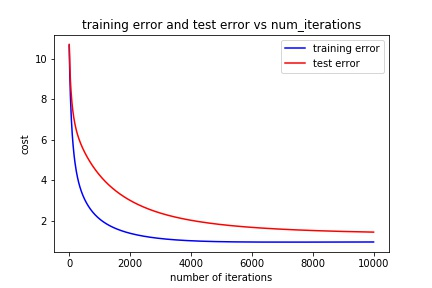
\includegraphics[width=0.45\textwidth]{latex_template/fig/LFMfig1.jpg}
    \caption{Training the Basic Latent Factor Model}
    \label{LFM1}
\end{figure}

The training error and test error both decrease when the program iterate more and more. Finally, they tend to be gentle and not change. There is a gap between training error and test error. We need both small training error and small gap. When our model has more parameters, the training error becomes smaller while the gap becomes larger. This is called overfitting. To decrease the gap and the effect of overfitting, we can increase the regularization term $\lambda$. However, if $\lambda$ is increased, the training error will also increase. So, there is a trade-off between fitting the training data well and generalizing to other dataset. We need to tune the parematers to find the best model. Figure \ref{LFM1} is the best solution we can get under basic latent factor model. The parameters are $\lambda_1 = 20$ and $\lambda_2 = 20$. The learning rate is 0.01. The number of latent factors are 100.

}

\item{
When we get $P$, $Q$, we can multiply the two matrices to get the rating predictions. $\hat{R} = P \cdot Q$. We find the first 10 highest ratings for each user in $\hat{R}$. This is our recommendation list for each user.
When calculating NDCG, we only calculate those users whose recommendation list is hit at least once.

}

\item{The experimental results are as following:}
\item{MAE= 1.0906}
\item{RMSE= 1.4390}
\item{precision = 0.02148}
\item{recall = 0.005281}
\item{F = 0.008478}
\item{NDCG = 0.5162}


\subsection{Latent Factor Model with Bias}
By using stochastic gradient descent, we can learn the parameters in the latent factor model with bias. For this experiment, $\lambda_1 = 0.2$, $\lambda_2 = 0.2$.

\item{The experimental results are :}
\item{MAE= 1.0818}
\item{RMSE= 0.8572}
\item{precision = 0.00613}
\item{recall = 0.005821}
\item{F = 0.003617}
\item{NDCG = 0.3793}


Full recommendation can be found in recommendation.csv. Here is a part of it.
\begin{lstlisting}
user_id	movies1	movies2	movies3	movies4	movies5	movies6	movies7	movies8	movies9	movies10
0	101	593	1197	1278	1967	2571	296	1080	3386	1208
1	46970	80906	89774	106782	6874	99114	48516	6025	6832	6754
2	914	5919	3703	720	5746	1124	1093	688	1587	3210
3	2078	3175	1080	345	1073	1282	176	3538	1057	2019
4	290	232	296	595	364	594	261	588	153	5265
5	818	209	835	330	291	314	358	41	87	251
6	49272	8360	4844	30812	1923	2640	45668	5991	1617	45517
7	592	235	34	231	2	587	141	432	282	208
8	5841	5447	1674	5451	3173	5952	5956	371	922	4993
9	8808	59421	98203	58559	51662	95510	4995	6155	72998	356
\end{lstlisting}


\subsection{Latent Factor Model with Temporal Biases}

\item{
Due to the limited size of our dataset, we set two bins to deal with the temporal effect. Some movies only have 1 or 2 ratings. If we set more bins, we don't have enough data. For every movie, we use the average time of its ratings to split the training dataset so that we can get two bins. In order to train the model well, we preprocess the training data again. We only reserve the movies who have at least 4 ratings. We do this because of the requirement of training.  
Through stochastic gradient descent, We train the model and get the parameters. The training process is shown in figure \ref{LFM3}.

\begin{figure}
    \centering
    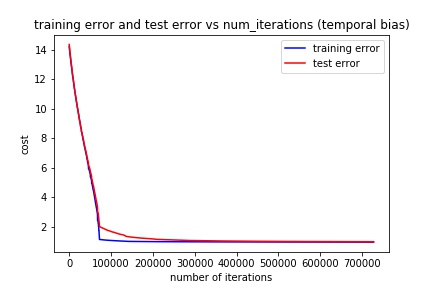
\includegraphics[width=0.45\textwidth]{latex_template/fig/fig6.jpg}
    \caption{Training the Latent Factor Model with Temporal Biases}
    \label{LFM3}
\end{figure}

In this case, the gap between train error and test error is very small. Ater tuning, the hyperparameters are $\lambda_1 = 4$, $\lambda_2 = 4$, $\lambda_3 = 4$, and $\lambda_4 = 4$. The learning rate is 0.002. The number of latent factors is 200.

After we get $P$, $Q$, $Bu$, $Bm$, we can do the prediction. There is a problem in prediction. We don't know when the user will watch the movie. So, the temporal effect can't work here. We take average over $b_{ti}$ to get $b_i$ and treat it as the bias of movie $i$. So, the prediction is $r_{xi} = \mu + b_x + average(b_{ti}) + p_x \cdot q_i$. Once we have the preditions, we can generate the recommendation list in a similar way.


}


\item{The experimental results are shown below:}
\item{MAE = 0.7830}
\item{RMSE = 0.9897}
\item{precision = 0.003114}
\item{recall = 0.0005303}
\item{F = 0.0009063}
\item{NDCG = 0.4296}


\section{Conclusions and Future Work}\label{sec:conclusions}
We use five models in our project. They are User-User Collaborative Filtering, Item-Item Collaborative Filtering, Basic Latent Factor Model, Latent Factor Model with Biases, and Latent Factor Model with Temporal Biases. We get the model and make predictions based on each model. We calculate many criteria to assess whether one model is good or not. We think the most appropriate criterion is RMSE. Watching a certain movie is a random event. One user can have a certain flavour, but he can't watch all movies under this genre. It is quite common that one user never watches movie A even if he watched movie B which is similar to A. There are often dozens of movies similar to movie B. The user may watch only one or two of them if he is not a movie fanatics. That is why precisions and recalls are very small in the experiments. Making a recommendation list for each user and assessing each model based on it is not a good idea. There is too much randomness in it. RMSE is more appropriate and stable to use as a criterion. Based on RMSE, the 4th model is the best model in our experiment. Due to the secondary preprocessing in the training process of the 5th model, its training set is smaller. So, its RMSE is a little lower than the 4th model.

We use 6 hours to train the 5th model on our laptop! The ilab of Rutgers CS is not stable. Jobs are easily to be killed on it. Due to the limitation of our computing resources, we can only choose small dataset. Due to the size of the dataset, we can't use complex model, such as the one mentioned in \cite{cf-temporal} and \cite{Koren-2008}.
\begin{equation}
    r_{xi}(t) = \mu + b_x(t) + b_i(t) + q_i^T(p_x(t) + |R(x)|^{0.5} \cdot \sum_{j \in R(x)}y_j)
\end{equation}

\begin{equation}
    b_x(t) = b_x + \alpha_x dev_x(t) + b_{xt}
\end{equation}

\begin{equation}
    b_i(t) = (b_i + b_{i,Bin(t)})c_x(t)
\end{equation}

If we have access to high performance computing clusters in the future, we can use larger dataset(tens of million) and more complex model above to build our movie recommendation system.

\section*{Acknowledgement}
Thanks to Han Wu, Ningyuan Zhang, Lemin Wu, and Zhe Huang.

\bibliographystyle{ACM-Reference-Format}
\balance
\bibliography{paper}

\end{document}






